\progres{
Rappel cours 6 :
\begin{itemize}
  \item Fin EDO et systèmes dynamiques
  \item TD fonctions de plusieurs variables + EDO \& syst. synamiques
\end{itemize}
Programme cours 7 :
\begin{itemize}
  \item Dernier chapitre : probabilités (procesus)
  \item Chaînes de Makov
  \item Distribution stationnaire / comportement en temps long
\end{itemize}
}

%-------------------------------------------------------------------------------
%-------------------------------------------------------------------------------
\section{Chaînes de Markov}  \label{sec:Proba-Markov}
%-------------------------------------------------------------------------------

\newcommand{\cM}{{chaîne de Markov}\xspace}
\newcommand{\CM}{{Chaîne de Markov}\xspace}
\newcommand{\per}{\text{per}}

\todo{Trouver un exemple simple de \cM servant de fil rouge.}

\paragraph*{Objectif.}
Etudier une suite de variable aléatoires $(X_0, X_1, \dots X_n, \dots)$ non indépendantes. L'indice $n$ se réfère souvent à un temps et une telle suite est alors appelées {\em processus stochastique} à temps discert ou {\em chaîne}. % On note alors $X = (X_t)_{t \geq 0}$.

\bigskip
On suppose ici que les variables $X_n$ sont toutes à valeurs dans un même ensemble $\Ecal$ fini ou dénombrable.

%-------------------------------------------------------------------------------
\subsection{Définitions et premières propriétés}  
%-------------------------------------------------------------------------------

%-------------------------------------------------------------------------------
\subsubsection{Hypothèse de Markov}

\begin{definition}[\CM]
  $X$ est une \cM si
  $$
  \Pr\{X_{n+1} = x_{n+1} \mid X_0 = x_0, X_1 = x_1, \dots X_n = x_n\} 
  = 
  \Pr\{X_{n+1} = x_{n+1} \mid X_n = x_n\}.
  $$
\end{definition}

\begin{proposition} \label{prop:loiConditionnalleEtatInitial}
  Si $X$ est un \cM, alors
  $$
  \Pr\{X_{n+1} = k \mid X_0 = i, X_n = j\} 
  = 
  \Pr\{X_{n+1} = k \mid X_n = j\}.
  $$
\end{proposition}

% {Démonstration de la proposition \ref{prop:loiConditionnalleEtatInitial}.}
\proof
On utilise le théorème des probabilités totales pour sommer sur toutes les valeurs intermédiaires
  \begin{align*}
    \Pr\{X_0 = i, X_n = j, X_{n+1} = k\}
    & = \sum_{x_1, x_2, \dots x_{n-1}}
    \Pr\{X_0 = i, X_1 = x_1, \dots X_{n-1} = x_{n-1}, X_n = j, X_{n+1} = k\} \\
    & = \sum_{x_1, x_2, \dots x_{n-1}}
    \Pr\{X_0 = i, X_1 = x_1, \dots X_{n-1} = x_{n-1}, X_n = j, X_{n+1} = k\} \\
    & = \sum_{x_1, x_2, \dots x_{n-1}}
    \Pr\{X_{n+1} = k \mid X_0 = i, X_1 = x_1, \dots X_{n-1} = x_{n-1}, X_n = j\} \\
    & \qquad \times \Pr\{X_0 = i, X_1 = x_1, \dots X_{n-1} = x_{n-1}, X_n = j\} \\
    & = \Pr\{X_{n+1} = k \mid X_n = j\} \\
    & \qquad \times \sum_{x_1, x_2, \dots x_{n-1}} \Pr\{X_0 = i, X_1 = x_1, \dots X_{n-1} = x_{n-1}, X_n = j\} \\
    & = \Pr\{X_{n+1} = k \mid X_n = j\} \Pr\{X_0 = i, X_n = j\}.
  \end{align*}
  Il suffit alors de diviser par $\Pr\{X_0 = i, X_n = j\}$ des deux côtés. 
\eproof

%-------------------------------------------------------------------------------
\subsubsection{Matrice de transition}

\begin{definition}[\CM homogène]
  Une \cM $X$ est homogène si
  $$
  \forall n \geq 1: \qquad 
  \Pr\{X_{n+1} = j \mid X_n = i\} = p_{ij} 
  \qquad (\text{indépendant de $n$}).
  $$
\end{definition}

\begin{definition}[Probabilité et matrice de transition]
  Soit $X$ un \cM homogène, on appelle probabilités de transition les probabilités :
  $$
  p_{ij} = \Pr\{X_1 = j \mid X_0 = i\}, \qquad \forall i, j \in \Ecal.
  $$
  On appelle de plus matrice de transition la matrice $P$ de terme général $p_{ij}$:
  $$
  P = [p_{ij}].
  $$
\end{definition}

\remarks
\begin{enumerate}
  \item On utilise la notation matricielle même si $\Ecal$ est infini (mais dénombrable).
  \item On rappelle que $P$ est une {\em matrice stochastique} : 
  $$
  \forall i \in \Ecal: \qquad \sum_{j \in \Ecal} p_{ij} = 1.
  $$
  En conséquence, chaque ligne $(p_{ij})_{j \in \Ecal}$ de $P$ définie une loi de probabilité.
\end{enumerate}

\begin{definition}[Transition de $n$ étapes]
  Soit $X$ un \cM homogène, on appelle probabilités de transition en $n$ étapes les probabilités :
  $$
  p_{ij}(n) = \Pr\{X_n = j \mid X_0 = i\}, \qquad \forall i, j \in \Ecal.  
  $$
\end{definition}

\begin{proposition} \label{prop:transitionNEtapes}
  Soit $X$ une \cM homogène, les probabilités $p_{ij}(n)$ sont les termes généraux de la matrice $P^n$ : 
  $$
  p_{ij}(n) = [P^n]_{ij}.
  $$
\end{proposition}

% {Démontration de la proposition \ref{prop:transitionNEtapes}.}
\proof
Le démonstration se fait par récurrence en supposant la propriété vraie au rang $n$. Il suffit alors de sommer sur tous les états précédents possibles : 
\begin{align*}
  p_{ik}(n+1) 
  & = \Pr\{X_{n+1} = k \mid X_0=i\} \\
  & = \sum_{k \in \Ecal} \Pr\{X_{n+1} = k, X_n = j \mid X_0=i\} \\
  & = \sum_{k \in \Ecal} \Pr\{X_n = j \mid X_0=i\} \; \Pr\{X_{n+1} = k \mid X_n = j, X_0=i\} \\
  & = \sum_{k \in \Ecal} \Pr\{X_n = j \mid X_0=i\} \; \Pr\{X_{n+1} = k \mid X_n = j\} \qquad (\text{cf exercice précédent})\\
  & = \sum_{k \in \Ecal} p_{ij}(n) \; p_{jk} = \sum_{k \in \Ecal} [P^n]_{ij} p_{jk} = [P^{n+1}]_{ik}.
\end{align*}
\eproof

\remark
La loi d'une \cM homogène $X$ est donc entièrement spécifiée par
\begin{itemize}
  \item sa matrice de transition $P$ et
  \item la distribution de sa valeur initiale $X_0$.
\end{itemize}

\paragraph*{Notation.}
Dans la suite on notera $\Pr_\mu$ la loi d'une \cM $X$
\begin{itemize}
  \item de distribution initiale $\mu$: $X_0 \sim \mu$ et
  \item de matrice de transition $P$.
\end{itemize}
On notera notamment $\Pr_i$ la loi de $X$ si $x_0 = i$, c'est à dire
$$
\Pr_\mu = \sum_{i \in \Ecal} \mu_i \Pr_i.
$$

\remark
On peut identifier la distribution $\mu$ à un vecteur ligne $\mu^\top$ (éventuellement infini). On peut alors écrire
$$
\Pr_\mu\{X_n = j\} 
= \sum_{i \in \Ecal} \Pr\{X_0 = i\} \Pr\{X_n = j \mid X_0 = i\}
= \sum_{i \in \Ecal} \mu_i p_{ij}(n)
= \sum_{i \in \Ecal} \mu_i [P^n]_{ij}
= [\mu^\top P^n]_j.
$$

%-------------------------------------------------------------------------------
\subsection{Distribution stationnaire}  
%-------------------------------------------------------------------------------

\begin{definition}
  Une distribution $\nu$ sur $\Ecal$ est dite \emph{invariante} pour la \cM $X$ si 
  $$
  \nu^\top P = \nu^\top.
  $$
\end{definition}

Les distributions invariantes jouent pour les chaînes de Markov un rôle analogue au point stationnaires en système dynamique : une fois atteinte, la distribution reste constante. Comme pour les systèmes dynamiques, la question est alors de savoir si elles seront atteintes et à quelle condition. Pour répondre à cette question, il nous faut d'abord définir une notion de convergence pour des distributions.

\begin{definition}[Convergence en loi]
  Une suite de v.a. $(Y_n)_{n \geq 0}$ à valeur dans $\Ecal$ converge en loi vers une distribution $\nu$ sur $\Ecal$ :
  $$
  (Y_n)_{n \geq 0} \overset{\Lcal}{\underset{n \to \infty}{\longrightarrow}} \nu
  $$
  si
  $$
  \forall i \in \Ecal: \qquad \lim_{n \to \infty} \Pr\{Y_n = i\} = \nu_i.
  $$
\end{definition}

\begin{proposition} \label{prop:convergenceEsperance}
  Si
  $$
  (Y_n)_{n \geq 0} \overset{\Lcal}{\underset{n \to \infty}{\longrightarrow}} \nu
  $$
  alors, pour toute fonction $f : \Ecal \mapsto \Rbb$ bornée, 
  $$
  \lim_{n \to \infty} \Esp(f(Y_n)) = \sum_{i \in \Ecal} \nu_i f(i)
  $$
  (c'est à dire $\lim_{n \to \infty} \Esp(f(Y_n)) = \Esp(f(Y))$ pour $Y \sim \nu$).
\end{proposition}

% {Démonstration de la proposition \ref{prop:convergenceEsperance}.}
\proof 
\begin{description}
  \item[$\Ecal$ fini :] la démonstration vient en intervertissant la somme et la limite (puisque $\Ecal$ est fini) : 
  $$
  \lim_{n \to \infty} \Esp(f(Y_n)) 
  = \lim_{n \to \infty} \left(\sum_{i \in \Ecal} \Pr\{Y_n = i\} f(i)\right)
  = \sum_{i \in \Ecal} \left(\lim_{n \to \infty} \Pr\{Y_n = i\} \right) f(i) 
  = \sum_{i \in \Ecal} \nu_i f(i).
  $$
  \item[$\Ecal$ infini dénombrable :] sans perte de généralité, on identifie $\Ecal$ à $\Nbb$. Comme pour le cas fini, on montre facilement que, pour tout $i$,
  $$
  \lim_{n \to \infty} \Pr\{Y_n \leq i\} = \Pr\{Y \leq i\}
  \qquad \Rightarrow \qquad 
  \lim_{n \to \infty} \Pr\{Y_n > i\} = \Pr\{Y > i\}.
  $$
  On note $M$ un majorant de $f$ (qui est bornée). On peut écrire que
  \begin{align*}
    \left|\Esp(f(Y_n)) - \Esp(Y)\right|
    & = \left|\sum_{j \geq 0} \Pr\{Y_n=j\} f(j) - \sum_{j \geq 0} \nu_j f(j)\right| \\
    & \leq \left|\sum_{j=0}^i \Pr\{Y_n=j\} f(j) - \sum_{j=0}^i \nu_j f(j)\right|
    + \left|\sum_{j > i} \Pr\{Y_n=j\} f(j) - \sum_{j > i} \nu_j f(j)\right| \\
%     & \leq \left|\sum_{j=0}^i \Pr\{Y_n=j\} f(j) - \sum_{j=0}^i \nu_j f(j)\right|
%     + \left|\sum_{j > i} \Pr\{Y_n=j\} f(j)\right| + \left|\sum_{j > i} \nu_j f(j)\right| \\
    & \leq M \sum_{j=0}^i \left|\Pr\{Y_n=j\} - \nu_j\right| + M \Pr\{Y_n > i\} + M \Pr\{Y > i\}.
  \end{align*}
  La suite de la preuve consiste à majorer chacun des trois termes par $\varepsilon/3M$. 
  \begin{itemize}
  \item On commence par utiliser le fait que, pour toute v.a. $U$ à valeur dans $\Nbb$, 
  $$
  \lim_{i \to \infty} \Pr\{Y_n > i\} = 0
  $$
  (puisque la somme $\sum_{n \in \Nbb} \Pr\{U = i\}$ converge). \\
  Donc, pour tout $\epsilon > 0$, il existe un $i$ et un $n_1^{(i)}$ tels que 
  \begin{align*}
  \Pr\{Y > i\} & < \epsilon / 3M, \\
  \text{et} \qquad 
  \forall n > n_1^{(i)}: \quad \Pr\{Y_n > i\} & < \epsilon / 3M.
  \end{align*}
  \item D'autre part, puisque $i$ est fini (i.e. en utilisant le résultat dans le cas fini), il existe de plus $n_2^{(i)}$ tel que 
  $$
  \forall n > n_2, \; \forall j \leq i: \quad \left|\Pr\{Y_n=j\} - \nu_j\right| < \frac\epsilon{3M(i+1)}.
  $$
  \end{itemize}
  On a donc, 
 \begin{align*}
   \forall n > \max(i, n_1^{(i)}, n_2^{(i)}): \qquad 
   \left|\Esp(f(Y_n)) - \Esp(Y)\right| \leq \frac{M\epsilon}{3M} \underset{=1}{\underbrace{\sum_{j=0}^i \frac1{i+1}}} + \frac{M\epsilon}{3M} + \frac{M\epsilon}{3M} = \epsilon.
  \end{align*}
\end{description}
\eproof

\remarks
\begin{enumerate}
\item Si $\Ecal$ est fini, la proposition \ref{prop:convergenceEsperance} nous assure par exemple que, si $(Y_n)_{n \geq 0}$ converge en loi vers $\nu$ et que $Y \sim \nu$, on a, en prenant respectivement $f(x) = x$ et $f(x) = x^2$, 
$$
\lim_{n \to \infty} \Esp(Y_n) = \Esp(Y), \qquad
\lim_{n \to \infty} \Esp(Y_n^2) = \Esp(Y^2)
$$
et, par conséquent, $\lim_{n \to \infty} \Var(Y_n) = \Var(Y)$. 
\item Pour $\Ecal$ quelconque, en prenant $f(x) = \Ibb\{x \leq u\}$, on a $\Esp(f(Y_n)) = \Pr\{Y_n \leq u\}$ et donc, pour tout $u$, 
$$
(Y_n)_{n \geq 0} \overset{\Lcal}{\rightarrow} \nu
\qquad \Rightarrow \qquad
\lim_{n \to \infty} \Pr\{Y_n \leq u\} = \Pr\{Y \leq u\}.
$$
\end{enumerate}

\begin{definition}
  Une distribution $\nu$ sur $\Ecal$ est dite \emph{stationnaire} pour la \cM $X$ si il existe une distribution $\mu$ telle que 
  $$
  \lim_{n \to \infty} \mu^\top P^n = \nu.
  $$
  C'est à dire que la \cM $X$ de transition $P$ et de distribution initiale $\mu$ converge en loi vers $\nu$.
\end{definition}

\begin{proposition} \label{prop:stationnaireInvariante}
  Une distribution $\nu$ sur $\Ecal$ est stationnaire pour la \cM $X$ ssi elle est invariante.
\end{proposition}

% {Démonstration de la proposition \ref{prop:stationnaireInvariante}.}
\proof
\begin{description}
  \item[$\Leftarrow$ :] il suffit de prendre $\mu = \nu$ pour s'assurer que $\mu^\top P^n = \nu^\top P^n = \nu$ pour tout $n$. (La \cM est alors dite {\em stationnaire}.)
  \item[$\Rightarrow$ :] si $\nu$ est stationnaire alors il existe $\mu$ telle que $\mu^\top P^n$ converge vers $\nu$ (i.e. $\lim_{n \to \infty} [\mu^\top P]_j = \nu_j$), ce qui implique que $\mu^\top P^{n+1}$ converge également vers $\nu$, i.e.
  $$
  \lim_{n \to \infty} [\mu^\top P^{n+1}]_j = \nu_j.
  $$
  Or, par l'exercice précédent, en prenant $f(i) = p_{ij}$, on a
  $$
  \lim_{n \to \infty} [\mu^\top P^{n+1}]_j
  = \lim_{n \to \infty} \sum_{i \in \Nbb} [\mu^\top P^n]_i p_{ij}
  = \sum_{i \in \Nbb} \nu_i p_{ij}
  = [\nu^\top P]_j,
  $$
  soit $\nu^\top P = \nu^\top$.
\end{description}
\eproof


% %-------------------------------------------------------------------------------
% \subsubsection{Chaîne de Markov}
% %-------------------------------------------------------------------------------
% 
% On revient maintenant aux chaînes de Markov introduites à la section \ref{sec:MatStoch} et qui seront étudiées plus en détail à la section \ref{sec:Proba-Markov}.
% 
% \begin{definition}
%   Une chaîne de Markov homogène à espace fini est une suite de variables aléatoires $\{X(n)\}_{n \geq 0}$ à valeur dans $\Xcal$ (identifié à $\{1, \dots k\}$) non indépendantes mais telles que
%   $$
%   \Pr\{X(n+1) = j \mid X(0)=x_0, X(1) = x_1) \dots X(n) = i\}
%   = \Pr\{X(n+1) = j \mid X(n) = i\}
%   = p_{ij}.
%   $$
%   La matrice $P = [p_{ij}]$ est appelée matrice de transition de la chaîne de Markov.
% \end{definition}
% 
% La matrice $P$ est une matrice stochastique car tous ses éléments sont positifs ou nuls et leur somme en ligne vaut 1 : 
% $$
% \sum_{j = 1}^k p_{ij} = 1.
% $$
% 
% \begin{proposition}
%   Soit $\mu_0$ la distribution de $X(0)$ : $\mu_{0i} = \Pr\{X(0) = i\}$ et $mu_n^{\mu_0}$ la distribution de $X(n)$ sachant la distribution initiale $\mu_0$, on a 
%   $$
%   \mu_n^{\mu_0} = \mu_0 A^n 
%   $$
% \end{proposition}
% 
% \proof
% Par récurrence, partant de $\mu_1^{\mu_0} = A \mu_0$.
% \eproof
% 
% Comme pour les modèles de dynamique des populations, le comportement de la chaîne de Markov en temps long est gouverné par par celui de $A^n$ (et par $\mu_0$).
% 
% \begin{proposition}
%   Si $A$ est diagonalisable, ses valeurs propres sont aussi les valeurs propres de $A^\top$ et les vecteurs propres de $A^\top$ sont les vecteurs lignes de $P^{-1}$.
% \end{proposition}
% 
% \proof
%   Il suffit de remarquer que, puique $A = P D P^{-1}$, on a 
%   $$
%   A^\top 
%   = (P D P^{-1})^\top 
%   = (P^{-1})^\top D^\top  P^\top
%   = (P^{-1})^\top D P^\top 
%   $$
%   donc $A^\top$ est aussi diagonalisable et possède les même valeurs propres (contenues dans $D$) que $A$. Pour les mêmes raisons, les vecteurs propres de $A^\top$ sont les vecteurs colonnes de $(P^{-1})^\top$, c'est à dire les vecteurs lignes de $P^{-1}$.
% \eproof
% 
% \remark
% Si $A$ est diagonalisable et que $u$ est un vecteur propre de $A^\top$, il existe $\lambda$ tel que
% $$
% A^\top u  = \lambda u 
% \qquad \Leftrightarrow \qquad
% (A^\top u)  = \lambda u^\top 
% \qquad \Leftrightarrow \qquad
% u^\top A  = \lambda u^\top 
% $$
% $u^\top$ est appelé vecteur propre {\em à gauche} de $A$ (les vecteurs propres précédemment définis étant donc des vecteurs propres {\em à droite}). Cette remarque est notamment utile pour étudier les matrice stochastiques.
% 
% Le théorème de Perron-Frobénius donne des conditions garantissant que la distribution $\mu_n$ converge vers le vecteur propre (à gauche) associé à la valeur propre 1, quelque soit la distribution initiale $\mu_0$. Ces propriétés seront étudiées en détail à la section \ref{sec:Proba-Markov}.
% 
% %-------------------------------------------------------------------------------
% \paragraph*{Exemple.}
% Succession d'espèces d'arbres (R. Arditi)
% \dessin{\url{TreeSpeciesMC}}

%-------------------------------------------------------------------------------
\subsection{Comportement en temps long}  
%-------------------------------------------------------------------------------

\begin{proposition} \label{prop:perronFrobeniusCM}
%[Exercice 1.1.14+]
  Si $\Ecal$ est fini, $1$ est la plus grande valeur propre en module de $P$. \\
  Si $P$ est de plus régulière, $1$ la seule valeur propre de module 1 et est d'ordre de multiplicité 1 : elle donc la valeur propre dominante de $P$.
\end{proposition}

% {Démonstration de la proposition \ref{prop:perronFrobeniusCM}.}
\proof
\begin{enumerate}
 \item On montre facilement que 1 est valeur propre de $P$ (car $P$ est stochastique), donc $\lambda_1 \geq 1$.
 \item Soit $\lambda$ une valeur propre de $P$ et $v$ un vecteur propre associé, on a $P^n v = \lambda^n v$ où $P^n$ est stochastique (voir section \ref{sec:MatStoch}), donc les coordonnées de $P^n v$ sont bornées par la plus grande coordonnée de $v$, ce qui impose que $\lambda \leq 1$, donc $\lambda_1 \leq 1$.
 \item Le fait que $P$ soit régulière assure, par le théorème \ref{thm:perronFrobenius} de Perron-Frobenius, que $\lambda_1$ est la valeur propre unique de module 1, toutes les autres ayant des modules strictement inférieurs. 
\end{enumerate}
\eproof

\remark
Le théorème \ref{thm:perronFrobenius} de Perron-Frobenius nous assure que les vecteurs propres (à gauche et à droite) associés à $\lambda_1 = 1$ ont toutes leurs coordonnées positives. On a ainsi démontré que, pour $\Ecal$ fini, si $P$ est régulière, 
\begin{itemize}
  \item elle admet une unique distribution stationnaire $\nu$ et que $\nu_i > 0$ pour tout $i \in \Ecal$, 
  \item quelque soit la distribution initiale $\mu$, $\mu P^n \to \nu$, c'est-à-dire que $X_n$ converge en loi vers $\nu$.
\end{itemize}

\progres{
Rappel cours 7 :
\begin{itemize}
  \item Chaînes de Markov
  \item Probabilités et matrice de transition
  \item Distribution invariante et stationnaire
  \item Comportement en temps long et convergence vers une distribution stationnaire (redonner la proposition \ref{prop:perronFrobeniusCM})
\end{itemize}
Programme cours 8 :
\begin{itemize}
  \item Communication entre états
  \item Classification des états
  \item Quelques exemples de \cM (Wright-Fisher)
  \item Processus de branchement
\end{itemize}
}

\begin{definition}[Communication entre états]
  On dit qu'il existe un {\em chemin de $i$ vers $j$} (ou que $j$ est {\em accessible depuis $i$}) s'il existe $n \geq 0: p_{ij}(n) > 0$. \\
  S'il existe une chemin de $i$ vers $j$ et un chemin de $j$ vers $i$, on dit que $i$ et $j$ communique et on note $i \sim j$.
\end{definition}


\begin{proposition}  \label{prop:communicationEquivalence}
  La relation de communication 
  $$
  \Rcal(i, j) \Leftrightarrow \{\text{$i$ communique avec $j$}\}
  $$
  est une relation d'équivalence. 
\end{proposition}

\proof
$\Rcal$ vérifie les trois condition d'une relation d'équivalence : 
\begin{itemize}
  \item reflexivité: $\forall i \in \Ecal: \Rcal(i, i)$ en prenant $n = 0$, soit $P^0 = I$ ;
  \item symétrie : $\forall i, j \in \Ecal: \Rcal(i, j) \Rightarrow \Rcal(j, i)$ ;
  \item transitivité : $\forall i, j, k \in \Ecal: \Rcal(i, j), \Rcal(j, k) \Rightarrow \Rcal(i, k)$.
\end{itemize}
\eproof

\remark
$\Rcal$ définit donc des classes d'équivalences $\Ccal_1, \Ccal_2, \dots $, qui constituent une partition de $E$:
$$
\cup_{k \geq 0} \Ccal_k = \Ecal, \qquad \forall j \neq k: \quad \Ccal_j \cap \Ccal_k = \varnothing.
$$
Les classes $\Ccal_k$ sont appelées {\em classes de communication}.

\begin{definition}
  Une \cM est dite {\em irréductible} si elle admet une seule classe de communication.
\end{definition}

\remark
L'hypothèse de régularité de $P$ implique que $X$ est irréductible (puisque $\exists n: P^n > 0$) mais pas l'inverse, puisque les états peuvent tous communiquer pour des $n$ différents.


%-------------------------------------------------------------------------------
\exemple{[$\Ecal = \{0, 1\}$.]
On considère la \cM $X$ de matrice de transition 
$$
P = \left[\begin{array}{ccc}
      1 - p & & p \\
      q & & 1 - q 
    \end{array}\right]
$$
\begin{description}
  \item[$p = q = 0$ :] alors $P = I$ et toute distribution est stationnaire, mais $P$ n'est pas régulière et la loi de $X_n$ est la même que celle de $X_0$.
  \item[$0 < p, q < 1$ :] alors la seule distribution stationnaire est 
  $$
  \nu = \left[ \frac{q}{p+q} \;  \frac{p}{p+q} \right],
  $$
  et comme $P$ est régulière, $X_n$ converge en loi vers $\nu$ quelque soit la distribution initiale $\mu$.
  \item[$p = q = 1$ :] alors la seule distribution stationnaire est 
  $$
  \nu = \left[ \frac12 \;  \frac12 \right],
  $$
  mais comme $P$ n'est pas régulière, $X_n$ ne converge pas nécessairement vers $\nu$. \\En fait $X_n$ alterne entre les états $0$ et $1$ et ne converge en loi vers $\nu$ que si $\mu = \nu$ (et alors $X_n \sim \nu, \forall n$). Si $X_0 = 0$ ou $X_0 = 1$ (ou $\mu \neq \nu$), alors $X_n$ ne converge pas du tout.
\end{description}
}
 
%-------------------------------------------------------------------------------
\subsection{Classification des états}  
%-------------------------------------------------------------------------------

% Loi du nombre de visites d’un état transient, théorème ergodique pour les chaînes récurrentes à espace d’états fini. 

On cherche maintenant à établir une classification des comportements possibles d'une \cM. La notion de temps de retour est centrale pour effectuer cette description.

\begin{definition}[Temps de retour]
  Le temps de retour dans l'état $i$ est défini pour $X_0 = i$ par
  $$
  T_i := \min\{n : X_n = i\} \leq + \infty \qquad (\text{i.e. possiblement } + \infty).
  $$
\end{definition}

\begin{definition}[\'Etat récurrent]
  L'état $i$ est dit {\em récurrent} si $\Pr_i\{T_i < + \infty\} = 1$. Dans le cas contraire, $i$ est dit {\em transient}. \\
  L'état $i$ est dit {\em récurrent positif} s'il est récurrent et $\Esp(T_i) < + \infty$. Dans le cas contraire il est dit récurrent nul.
\end{definition}

% \begin{definition}[\'Etat transient]
%   L'état $i$ est transient si $\Pr_i\{T_i < + \infty\} = 1$.
% \end{definition}

\begin{definition}[Période d'un état]
  La période de l'état $i$ est le plus grand diviseur commun des temps de retour possible dans l'état :
  $$
  \per(i) = PGCD\{n: p_{ii}(n) > 0\}.
  $$
  Une \cM est dite {\em apériodique} si $\per(i) = 1$ pour tout $i$.
\end{definition}

\dessin{Dessiner qques graphes de transition de \cM avec ou sans période.}

\begin{proposition}[Cas $\Ecal$ fini]
  Si $\Ecal$ est fini, il n'existe pas d'état récurrent nul et il existe au moins un état récurrent positif.
\end{proposition}

\proof Non démontré. \eproof

\begin{proposition}
  Tous les états d'une même classe de communication sont de même nature (récurrent positif, récurrent nul, transient). \\
  Si $\Ecal$ est fini et $X$ irréductible, son unique classe de communication est récurrente positive.
\end{proposition}

%-------------------------------------------------------------------------------
\exemple{[Modèle de Wright-Fisher]
  Le modèle de Wright-Fisher est un modèle classique en génétique des populations. On y considère les générations successive d'une population de taille fixe $N$ de reproduction non-sexuée. Parmi ces $N$ individus, $x$ sont porteurs de l'allèle $A$ (et $N-x$ sont porteurs de l'allèle $B$) d'un gène donné. On s'intéresse au processus $X = (X_n)_{n \geq 0}$ où
  $$
  X_n = \text{nombre d'individus porteurs de l'allèle $A$ à la génération $n$}
  $$
  en supposant que, à chaque génération, chacun de $N$ nouveaux individus tire indépendamment et uniformément son parent parmi la génération précédente (et hérite de son allèle). 
  \begin{description}
    \item[Probabilité de transition.] Un individu de la génération $n+1$ a donc un probabilité $x_n/N$ de porter l'allèle $A$. Les individus étant indépendant, on a
    $$
    (X_{n+1} \mid X_n=x) \sim \Bcal(N, x/N).
    $$
    La probabilité de transition vaut donc
    $$
    p_{ij} = \binom{N}{j} \left(\frac{i}N\right)^j \left(\frac{N-i}N\right)^{N-j}.
    $$
    \item[Classification des états.] Les états se répartissent en trois classes
    $$
    \Ccal_1 = \{0\}, \qquad \Ccal_2 = \{N\}, \qquad \Ccal_3 = \{1, \dots, N-1\}.
    $$
    Les classes $\Ccal_1$ et $\Ccal_2$ sont absorantes. La \cM finira nécessairement par atteindre l'une d'entre elles, $\Ccal_3$ est donc transiente.
    \item[Probabilité de fixation.] Il reste à savoir quel état absorbant sera atteint en premier. Notons $q_i$ la probabilité d'atteindre l'état $x=N$ (avant l'état $x=0$) en partant de $X_0 = i$. On a 
    $$
    q_0 = 0, \qquad q_N = 1.
    $$
    Pour les autres valeurs de $i$, en décomposant les chemins allant de $i$ à $N$ : 
    \begin{itemize}
      \item soit $i \to N$ en une étape, 
      \item soit $i \to j \notin \{0, N\}$ en une étape, puis $j \to N$ en un nombre indéterminé d'étapes, 
    \end{itemize}
    on peut écrire que :
    $$
    q_i = \sum_{j=1}^{N-1} p_{ij} q_j + p_{iN}
    $$
    et vérifier que $q_i = i/N$ satisfait cette équation, en effet :
    \begin{align*}
      \sum_{j=1}^{N-1} p_{ij} \frac{j}N + p_{iN}
      & = \sum_{j=1}^{N-1} \binom{N}{j} \left(\frac{i}N\right)^j \left(\frac{N-i} N\right)^{N-j} \frac{j}N + \left(\frac{i}N\right)^N \\
%       & = \binom{N}{j} \left(\frac{N-i} N\right)^N \sum_{j=1}^{N-1} \left(\frac{i}N\right)^j \left(\frac{N-i} N\right)^{-j} \frac{j}N + \left(\frac{i}N\right)^N \\
      & = \sum_{j=1}^{N-1} \binom{N-1}{j-1} \left(\frac{i}N\right)^j \left(\frac{N-i} N\right)^{N-j} + \left(\frac{i}N\right)^N \\
      & = \frac{i}N \sum_{k=0}^{N-2} \binom{N-1}{k} \left(\frac{i}N\right)^k \left(\frac{N-i} N\right)^{N-1-k} + \left(\frac{i}N\right)^N \\
      & = \frac{i}N \left[\left(\frac{i}N + \frac{N-i}N\right)^{N-1} - \left(\frac{i}N\right)^{N-1}\right] + \left(\frac{i}N\right)^N \\
      & = i/N.
    \end{align*}
    (On ne démontre pas ici que $q_i = i/N$ est l'unique solution.) La probabilité de fixation de l'allèle $A$ est donc $i/N$ (et celle de l'allèle $B$ est $(N-i)/N$).
  \end{description}
  
}

%-------------------------------------------------------------------------------
\exemple{[Marche aléatoire sur $\Zbb$]
  On considère la \cM $X$ à valeur dans $\Ecal = \Zbb$, de probabilités de transition
  $$
  p_{i, j} = \left\{\begin{array}{rl}
                    p & \text{si } j = i+1, \\
                    1 - p & \text{si } j = i-1, \\
                    0 & \text{sinon.}
                    \end{array}\right.
  $$
  \begin{description}
    \item[$p = 0$ ou $p = 1$:] chaque singleton constitue une classe transiente (la \cM y passe une fois et une seule).
    %
    \item[$p \in (0, 1)$:] $X$ est irréductible ($\Zbb$ forme une unique classe de communication). En notant $E_n$ le déplacement $X_n - X_{n-1}$, on voit que les $E_n$ sont iid à valeur dans $\{-1, +1\}$ et de loi
    $$
    \Pr\{E_n = 1\} = p = 1 - \Pr\{E_n = -1\}.
    $$
    On a notamment
    \begin{align*}
      \Esp(E_n) & = n (2p - 1) =: m, \\
      \Var(E_n) & = \Esp(E_n^2) - (2p - 1)^2 = 1 - (4p^2 - 4p + 1) = 4p(1-p) =: s^2.
    \end{align*}
    Puisque
    $$
    X_n = X_0 + \sum_{i=1}^n X_i,
    $$
    la loi des grands nombre nous assure que 
    $$
    \lim_{n \to \infty} \frac{X_n}n = \lim_{n \to \infty} \left(\frac{X_0}n + \frac1n \sum_{i=1}^n X_i\right) = m.
    $$
    Plus précisémment encore, le théorème central limite nous assure (puisque $X_0 /n \to 0$) que
    $$
    \frac{\sqrt{n}}{s}\left(\frac{X_n}n - m\right) \overset{\Lcal}\rightarrow \Ncal(0, 1),
    $$
    c'est-à-dire que
    $$
    \lim_{n \to \infty} \Pr\left\{\frac{\sqrt{n}}{s}\left(\frac{X_n}n - m\right) \in [a, b]\right\} = \Pr\{\Ncal(0, 1) \in [a, b]\}.
    $$
    \item[$p \in (0, 1)$ et $p \neq 1/2$:] alors $\Esp(X_n) = nm$ et
    $$
    \frac{\sqrt{n}}{s}\left(\frac{X_n}n - m\right) \in [a, b]
    \qquad \Leftrightarrow \qquad
    X_n \in [nm + \sqrt{n}as, nm + \sqrt{n}bs].
    $$
    La trajectoire est dite {\em balistique} (elle s'écarte de son origine à vitesse linéaire) et son écart type $\sqrt{\Var(X)}$ croît seulement en $\sqrt{n}$. $X_n$ tend vers $+\infty$ si $p > 1/2$ et vers $-\infty$ si $p < 1/2$ et la \cM est transiente.
    \item[$p = 1/2$:] on parle alors de marche aléatoire {\em symétrique}. Dans ce cas, $m=0$ et $s^2 = 1$, donc
    $$
    \frac{\sqrt{n}}{s}\left(\frac{X_n}n - m\right) \in [a, b]
    \qquad \Leftrightarrow \qquad
    X_n \in [\sqrt{n}a, \sqrt{n}b].
    $$
    $X_n$ si situe alors typiquement à une distance $\sqrt{n}$ de son origine. \\
    On peut montrer que $X$ est récurrente nulle : la \cM repasse un nombre infini de fois dans chaque état, mais les temps de passage sont de plus en plus espacés.
  \end{description}
  $$
  \begin{array}{cc}
    p = 1/3 & p = 1/2 \\
    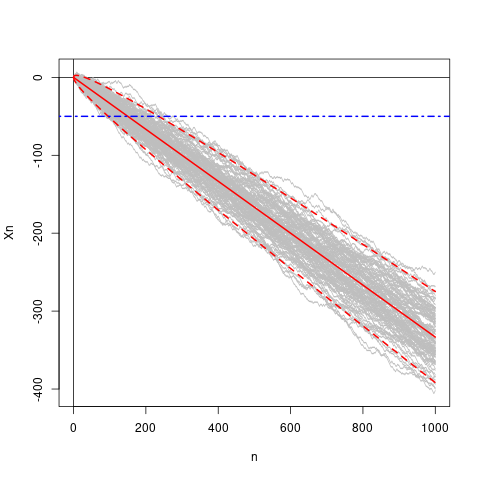
\includegraphics[width=.4\textwidth, trim=0 0 20 50, clip=]{MarcheAleatoire-p33} & 
    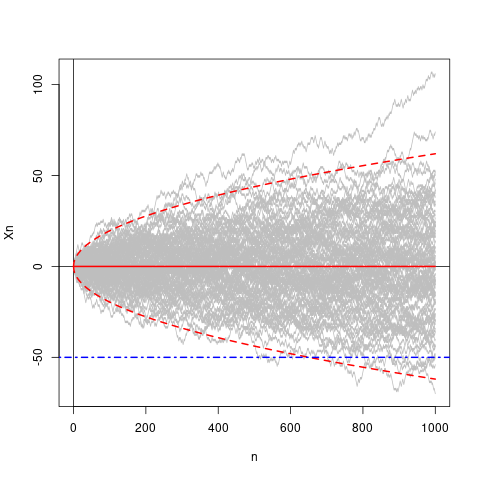
\includegraphics[width=.4\textwidth, trim=0 0 20 50, clip=]{MarcheAleatoire-p50} 
  \end{array}
  $$
}

%-------------------------------------------------------------------------------
%\subsection{Théorème ergodique}  
%-------------------------------------------------------------------------------

\begin{theorem}[Théorème ergodique]
  Si $X$ est une \cM irreductible et récurrente positive, alors 
  \begin{itemize}
   \item $X$ admet une unique distribution stationnaire $\nu$,
   \item $X$ est ergodique, c'est à dire que, pour toute distribution initiale $\mu$, on a
   $$
   \Pr_\mu\left\{\lim_{n \to \infty} \frac1n \left|\{1 \leq k \leq n: X_k = i\}\right| = \nu_i\right\} = 1,
   $$
   \item si de plus $X$ est apériodique alors $X$ converge en distribution vers $\nu$ : 
   $$
   \lim_{n \to \infty} \Pr_\mu\{X_n = i\} = \nu_i.
   $$
  \end{itemize}
\end{theorem}

\remarks
\begin{enumerate}
 \item Ce théorème est plus fort que la convergence en loi car il assure que la trajectoire de $X = (X_n)_{n \geq 0}$ elle même passe par chaque état $i$ un nombre de fois proportionnelle à $\nu_i$.
 \item La convergence en loi n'est garantie que dans le cas apériodique.
\end{enumerate}


%-------------------------------------------------------------------------------
\exemple{[$\Ecal = \{0, 1\}$]
\begin{description}
  \item[$p = q = 0$ :] la chaîne possède 2 classes récurrente ($\{0\}$ et $\{1\}$). Elle reste en fait constante et toute mesure $\nu$ est invariante.
  \item[$p = 0$ et $q \neq 0$ :] la chaîne possède une classe récurrente ($\{0\}$) et une classe transiente ($\{1\}$). La chaîne est 'absorbée' par l'état $0$ en un temps fini et la seule distribution invariante est $\nu = [1 \; 0]$.
  \item[$p = q = 1$ :] la chaîne est irréductible (on vérifie que $P^2 = I$) et récurrente positive, donc elle est ergodique (chaque état est visité la moitié du temps) mais elle est périodique et ne converge pas en loi.
  \item[$p + q = 1$ et $pq < 1$:] la chaîne est irréductible, récurrente positive et apériodique donc elle est ergodique et converge en loi vers $\nu$.
\end{description}
}

